\section{Problemstellung}

Diese Arbeit beschäftigt sich mit dem Problem der zeitnahen und transparenten Rückverfolgung von Chargen und Einzelprodukten über den gesamten Verlauf der Wertschöpfungskette. Lebensmittelsicherheit ist strategisch für die Volksgesundheit und das Wohlbefinden der Gesellschaft. Der öffentliche Druck auf Hersteller für eine ausreichende Kennzeichnung von Produkten und ihren Bestandteilen wird stetig größer.\\

Grundlage zur Chargenrückverfolgung ist die EU-Verordnung 178/02 (insbesondere Artikel 18 und 19), die die Notwendigkeit beschreibt, dass jeder in einer Lieferkette befindliche Teil der Lieferkette dafür verantwortlich ist nachzuweisen, von wem er seine Waren bezogen und an wen er seine Waren geliefert hat.\cite{EU2002}\\

Zum jetzigen Zeitpunkt findet eine Chargenrückverfolgung fast ausschließlich durch einen Datei-Austausch bzw. eine zentrale Datenbank je Teilnehmer der Lieferkette statt. Dabei müssen Informationen für einen mehrstufigen Produktionsporozess bereitgestellt und verarbeitet werden. In der Fleischwarenindustrie zum Beispiel existieren weit über 140 unterschiedliche Austauschformate zwischen den Teilnehmern der Lieferkette. So basiert die Echtheit der ausgetauschten Daten im Zweifel auf dem Glaube der Marktteilnehmer.\\



Die Fragestellung der Arbeit lautet daher: Kann die Blockchain Technologie den Prozess der Rückverfolgung von Chargen und/oder individuellen Produkten von der Rohstoffgewinnung bis hin zum letztendlichen Verkauf an den Endverbraucher für alle Teilnehmer der Wertschöpfungskette transparenter und sicherer gestalten?\\

Die Kernidee hinter der Blockchain-Technologie ist es einen Intermediär zu substituieren, der nur eingesetzt wurde um eine neutrale Vertrauensbildung zu ermöglichen. \ac{dlt} verfolgt dabei den Ansatz die Vertrauensbildung, den Ablauf von Transaktionen und deren sichere Festschreibung mit mathematischen und kryptographischen Methoden zu realisieren. Im Kontrast zum konventionellen Intermediär, welcher durch eine dritte Person oder Institution wie z.B. eine Bank oder einen Notar repräsentiert wird.\\

Für das Problem der Einigkeit über den Zustand eines Werts innerhalb der Blockchain sind zwei generelle Verfahren etabliert. Die \ac{pow} und \ac{pos} genannten Algorithmen nutzen unterschiedliche Ansätze um Konsens innerhalb eines Netzwerks zu bilden und so Vertrauen herzustellen. Beide Verfahren haben ihre Vor- und Nachteile.\\

Prozesse die einen transaktionalen Charakter besitzen und oft auch ein oder mehrere Vermittlerstellen zwischengeschaltet haben würden sich Ideal für den Einsatz von Blockchain Technologie eignen. Fehlende Standards und generelle Unsicherheit verhindern allerdings den flächendeckenden Einsatz der Technologie.\\

Abbildung \ref{fig:statista-huerden-blockchain-2016} zeigt die Ergebnisse einer Umfrage des Fachmagazins Cofinpro zum Thema \glqq Wo sehen Sie Hürden für die Blockchain-Technologie?\grqq~. So scheinen die mit Abstand größten Einstiegsbarrieren fehlende Standards und rechtliche Regelungen zu sein.

\begin{figure}[h!]
	\centering
	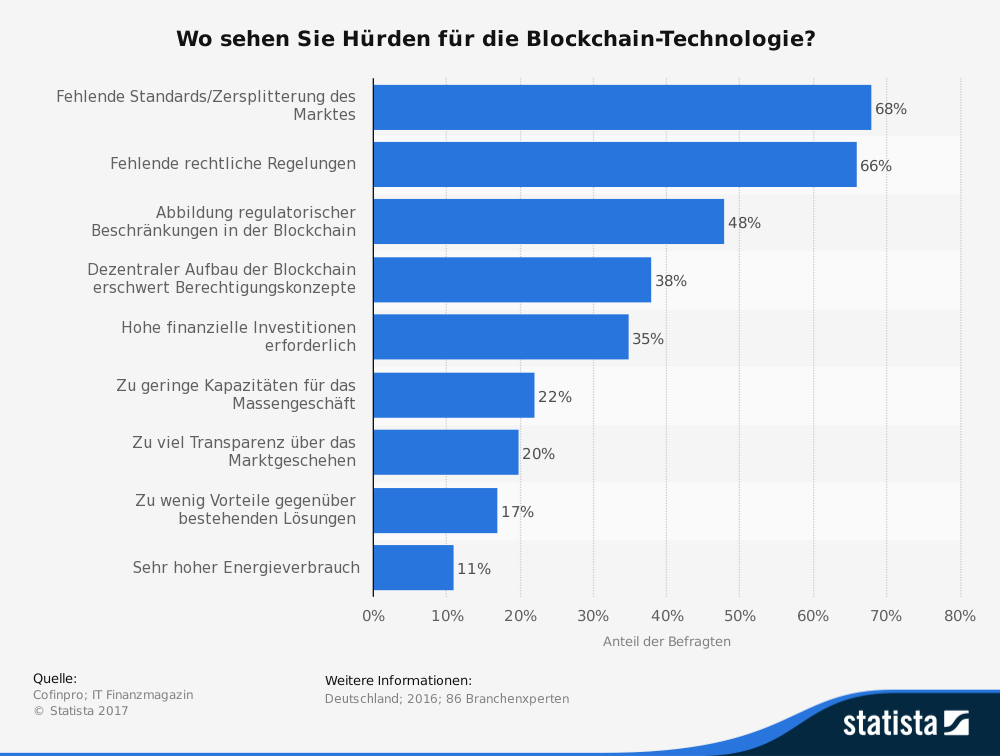
\includegraphics[width=0.7\linewidth]{pictures/Statista-Huerden-Blockchain-2016}
	\caption[Statista Blockchain Umfrage]{Cofinpro - Wo sehen Sie Hürden für die Blockchain Technologie? \cite{Cofinpro}}
	\label{fig:statista-huerden-blockchain-2016}
\end{figure}


%Soll die Blockchain Technologie zum Einsatz kommen gibt es offene Fragen. Eine Blockchain ist keine Silberkugel für sämtliche betriebswirtschaftliche Prozesse. Viel mehr kann eine Blockchain als Skalpell dienen um präzise ein bestimmtes Problem zu lösen.\\

%\begin{itemize}
%	\item Technologie ist so neu und frisch verfügbar im Industriekontext
%	\item Ermittlung und Definition möglicher Geschäftsprozesse der Energiewirtschaft
%	\item Vorhandene Lösungen am Markt vergleichen für den Einsatz
%	\item Mehrwert eines DLT-basierten Geschäftsprozesses herausarbeiten
%	\item Spieltheorie neue Geschäftsfelder Blockchain
%\end{itemize}

%Video [Wir und die Blockchain (The Blockchain and Us) (2017) - Deutsche Synchronfassung/German version - YouTube](\url{https://www.youtube.com/watch?v=x2mKDWsNijo})

% konkrete Beschreibung des Problems

\newpage
